\documentclass[11pt]{article}
\usepackage{amsmath, amssymb}
\usepackage{geometry}
\usepackage{graphicx}

% Set page margins
\geometry{margin=1in}

\title{Partial Differential Equations: \\ Heat Conduction and Materials}
\author{Yang transcribed by Handwriting of Prof Langemann}
\date{07.11.2023}

\begin{document}

\maketitle

\section*{PDE: Partial Differential Equations}

\subsection*{I.1. Diffusion and Heat Conduction}
Consider a position \( \vec{x} \in \Omega \subseteq \mathbb{R}^d \) within the domain \( \Omega \) (open!),
where \( d=1 \) corresponds to a channel or wire, \( d=2 \) to a plate, and \( d=3 \) to real space.
For time \( t \geq 0 \), let \( u = u(t, \vec{x}) \) represent the concentration or temperature, which are two independent physical quantities.
Let \( \vec{I} = \vec{I}(t,\vec{x}) \in \mathbb{R} \) denote the material or thermal flux.

\textbf{Constitutive Equation / Material Equation:}
\begin{enumerate}
\item Homogeneous (independent of \( \vec{x} \)) isotropic (independent of the direction) materials, the flux \( \vec{I} \) is given by \( \vec{I} = -a \nabla u \), where \( a > 0 \) represents the heat conduction or diffusion coefficient.
\item Inhomogeneous isotropic material, \( \vec{I} = -a(\vec{x}) \nabla u \), where \( a(\vec{x}) \geq \epsilon > 0 \) for some \( \epsilon \).
\item Inhomogeneous anisotropic material.
\end{enumerate}



\section*{Inhomogeneous Anisotropic Material}

For an inhomogeneous anisotropic material, the thermal or material flux \( \vec{I} \) is given by:
\[ \vec{I} = -A(\vec{x}) \nabla u \]
with the matrix \( A(\vec{x}) \in \mathbb{R}^{d \times d} \) satisfying:
\[ \vec{v}^T A(\vec{x}) \vec{v} > 0 \quad \text{for all} \quad \vec{v} \neq \vec{0} \]
which implies that \( A(\vec{x}) \) is positive definite.

Furthermore, we assume that:
\[ \vec{I} \cdot \nabla u < 0 \quad \text{for all} \quad \nabla u \neq \vec{0} \]
This is usually the case for physical systems where the flux tends to reduce the gradient (e.g., heat flows from hot to cold regions).

We also consider the spectrum of \( A(\vec{x}) \), denoted as \( \text{spec} \, A(\vec{x}) \), to satisfy:
\[ \text{spec} \, A(\vec{x}) \geq \varepsilon > 0 \]

\textbf{Remark:}
The symmetry of \( A(\vec{x}) \) is considered with respect to its action on the gradient vector \( \nabla u \). For a vector \( \nabla u = \begin{pmatrix} 1 \\ 0 \end{pmatrix} \), the resulting flux \( \vec{I} \) will be proportional to the first column of \( A(\vec{x}) \), specifically \( \vec{I} = - \begin{pmatrix} a_{11} \\ a_{21} \end{pmatrix} \) for the given gradient.


\section*{Continuity Equation}

Considering a sub-domain \( O \subseteq \Omega \), the total material or energy in \( O \) is denoted by:
\[ E = \int_O u \, da \]

For dimension \( d = 2 \), the change of \( E \) over time is:
\[ \frac{dE}{dt} = \frac{d}{dt} \int_O u \, da = \int_O \frac{\partial u}{\partial t} \, da \]

On the other hand, the change of \( E \) due to the flow across the boundary is given by:
\[ \frac{dE}{dt} = -\int_{\partial O} \vec{I} \cdot \vec{n} \, ds = -\int_O \nabla \cdot \vec{I} \, da \]
where \( \vec{I} \) is the flow vector and \( \vec{n} \) is the outward normal vector at the boundary \( \partial O \).

Therefore, the continuity equation can be expressed as:
\[ \int_O \frac{\partial u}{\partial t} \, da = -\int_O \nabla \cdot \vec{I} \, da \]
for every \( O \) independent of the material, leading to:
\[ \frac{\partial u}{\partial t} + \nabla \cdot \vec{I} = 0 \]

\begin{figure}
    \centering
    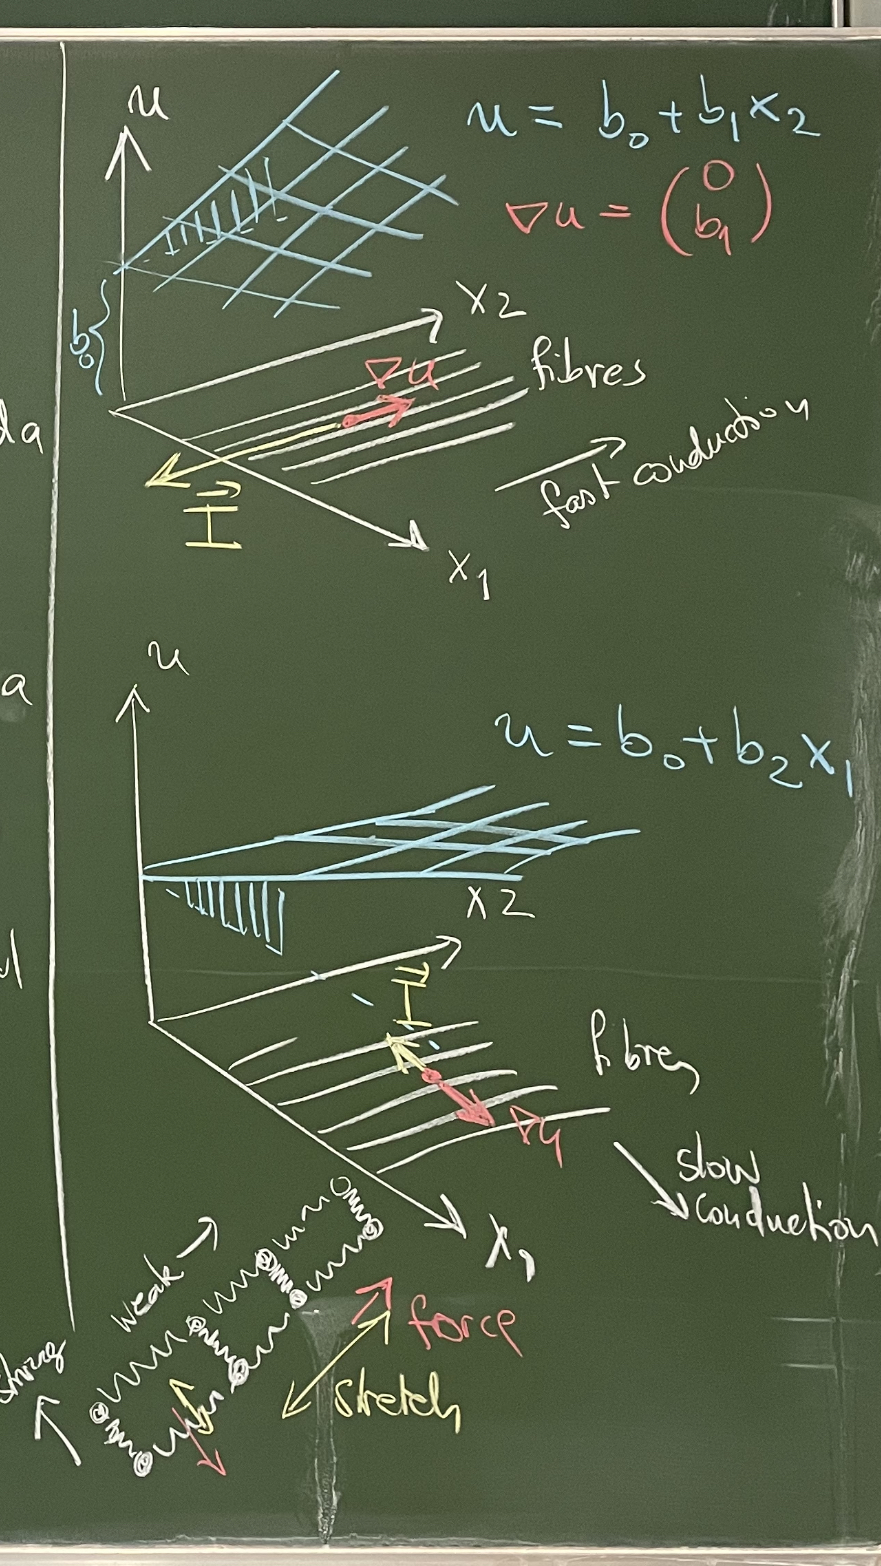
\includegraphics[width=0.5\linewidth]{IMG_2734.jpeg}
    \caption{heat conduction and force distribution}
    \label{fig:enter-label}
\end{figure}

\newpage
\date{15.11.2023}
\section*{PDE}


\begin{document}

\section*{Heat Diffusion Equation}

Domain $\Omega$

Boundary $\partial\Omega = \Gamma_1 \cup \Gamma_2$ and $\Gamma_1 \cap \Gamma_2 = \emptyset$

$\Gamma_1 \in \partial\Omega$ - given flux (Neumann BC - natural BC)

$\Gamma_2 \in \partial\Omega$ - $u = q$ (fixed value, Dirichlet Boundary Condition)

\subsection*{Full initial and boundary value problem (IBVP)}

PDE $\frac{\partial u}{\partial t} - \nabla \cdot \left( A(x) \nabla u \right) = f(x,t)$ for $x \in \Omega, t > 0$

$u(x,t) = g(x,t)$ for $x \in \Gamma_1, t > 0$

$n^T \left( A(x) \nabla u \right) = p(x,t)$ for $x \in \Gamma_2, t > 0$

$u(0,x) = u_0(x)$ for $x \in \Omega$

\subsection*{Mass conservation / energy conservation}

Total mass / total energy $E = \int_{\Omega} u \, da$

Change $\frac{dE}{dt} = \int_{\Omega} \frac{\partial u}{\partial t} \, da = \int_{\Omega} \nabla \cdot \left( A(x) \nabla u \right) \, da + \int_{\Omega} f \, da$

$= \int_{\partial\Omega} \left( A(x) \nabla u \right) \cdot n \, ds + \int_{\Omega} f \, da$

Flow over $\partial\Omega$ not convoluted with $\Gamma_1$

$p$ in $\Gamma_2$

If only Neumann BC are used, then

$\frac{dE}{dt} = \int_{\Gamma_2} p \, ds + \int_{\Omega} f \, da$

Transport over the boundary $\Gamma_2$ and internal sinks and sources

Input/output of $\Gamma_2$ BC


\section*{Stationary Case}

That is, \( \frac{\partial u}{\partial t} = 0 \)

Only for \( p(x,t) = p(x) \), \( q(x,t) = q(x) \) and \( f(x,t) = f(x) \)

Then, 
\[
-\nabla \cdot (A(x) \nabla u) = f(x) \text{ in } \Omega
\]
\[
u(x) = q(x) \text{ on } \Gamma_1
\]
\[
n^T(A(x) \nabla u) = p(x) \text{ on } \Gamma_2
\]

For \( \Gamma_2 \), i.e., \( \Gamma_2 = \partial \Omega \) we find
\[
\int_{\Omega} f \, da = -\int_{\Omega} \nabla \cdot (A(x) \nabla u) \, da = 
\]
\[
= -\int_{\Gamma_2} n^T (A(x) \nabla u) \, ds = -\int_{\Gamma_2} p \, ds
\]

Because 
\[
\int_{\Omega} f \, da + \int_{\Gamma_2} p \, ds = 0
\]
\( p \) production/ sink inside \( \Omega \) \\
Transport over the boundary

\subsection*{Oscillations/Elasticity}

\begin{figure}[h!]
\centering
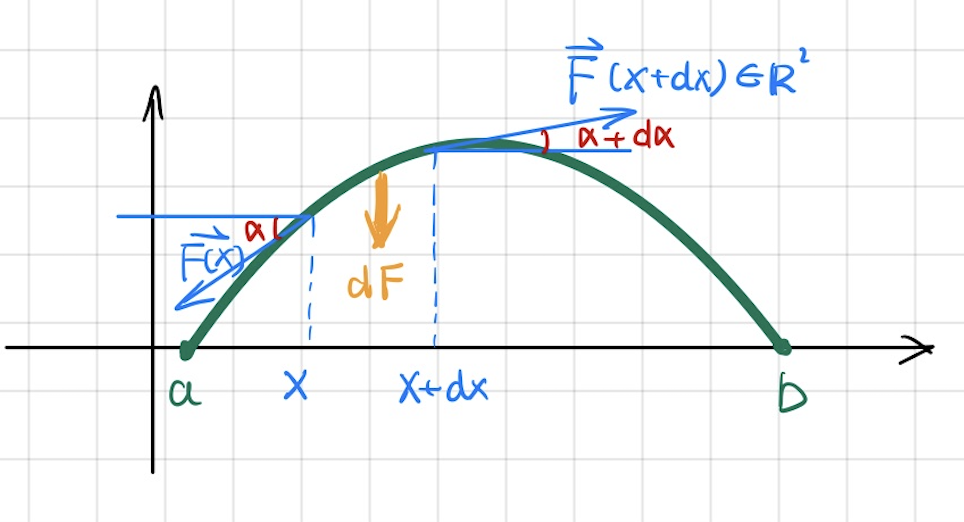
\includegraphics[width=0.6\textwidth]{graph.png}
\caption{Elasticity graph.}
\end{figure}

\( F(x + dx) - F(x) = P \)

Vertical components are 
\[
|F(x)| \sin(\alpha) = P \cos(\alpha) \text{ etc.}
\]

Resulting force \( dF \) is
\[
P (\sin(\alpha + d\alpha) - \sin(\alpha)) \approx P (\tan(\alpha + d\alpha) - \tan(\alpha)) 
\]
\[
= P (u'(x + dx) - u'(x))
\]

By Taylor \( P (u'(x) + u''(x)dx + O(dx^2) - u'(x)) \)

Thus \( dF = P u''(x) dx \) force acting on the unit

Now \( u(x,t) = u(x) \)

Newton's 2nd law \( u''(x) = \frac{dF}{P dx} = \frac{P u''(x) dx}{P dx} \)


\section*{One Dimensional Wave Equation}

Initial Boundary Value Problem (IBVP) for the 1d wave equation:

\[
\begin{cases}
S u_{tt} = P u_{xx} + f(t,x), & \text{for } x \in (a,b), t > 0 \\
u(t,a) = u(t,b) = 0, & \text{for } t > 0 \\
u(0,x) = u_0(x), & \text{for } x \in (a,b) \\
u_{t}(0,x) = v_0(x), & \text{for } x \in (a,b)
\end{cases}
\]

where \( S \) and \( P \) are constants, and \( f(t,x) \) is a given function.

BC denotes Dirichlet boundary condition, which is attached here.

IC represents initial conditions for position and velocity of the system.

\subsection*{Potential Energy of the Deformed String}
\[
dE_{pot} = P \left( \sqrt{1 + u_{x}^2} - 1 \right) dx \approx P \left( \frac{1}{2} u_{x}^2 \right) dx
\]

Using Taylor expansion, we get:
\[
dE_{pot} = \frac{P}{2} u_{x}^2 dx
\]

\subsection*{Energy Balance of the String}

The total energy \( E \) of the string is the sum of potential and kinetic energy:
\[
E = E_{pst} + E_{kin} = \int_{a}^{b} \frac{P}{2} u_{x}^2 dx + \int_{a}^{b} \frac{S}{2} u_{t}^2 dx
\]

The change in energy with respect to time is given by:
\[
\frac{dE}{dt} = \int_{a}^{b} P u_{x} u_{xt} dx + \int_{a}^{b} S u_{t} u_{tt} dx
\]

Using the chain rule and partial integration, we obtain:
\[
\int_{a}^{b} u_{x} u_{xt} dx = u u_{t} \Big|_{a}^{b} - \int_{a}^{b} u u_{xtt} dx = -\int_{a}^{b} u u_{xtt} dx
\]
since \( u(t,a) = u(t,b) = 0 \) due to Dirichlet boundary conditions.

\subsection*{Remarks}

If \( t \neq 0 \), then the change in energy with respect to time is:
\[
\frac{dE}{dt} = \int_{a}^{b} S u_{t} u_{tt} dx
\]

In the stationary state where \( u_{tt} = 0 \), we have \( P u_{xx} = 0 \) in \( (a,b) \).



\subsection*{Remarks on the Two-Dimensional Wave Equation}

Considering a membrane representing a two-dimensional material without resistance against bending. The force applied is \( f(t,x) \).

\[
S u_{tt} = P (\Delta u_{xx} + \Delta u_{yy}) + f
\]

or in a more compact form,

\[
S u_{tt} = P \Delta u + f
\]

where \( S \) and \( P \) are constants related to the properties of the membrane, \( \Delta \) is the Laplacian operator representing the sum of second partial derivatives in the spatial dimensions, and \( f \) is a function representing the external force applied to the membrane.

\begin{figure}[h!]
\centering
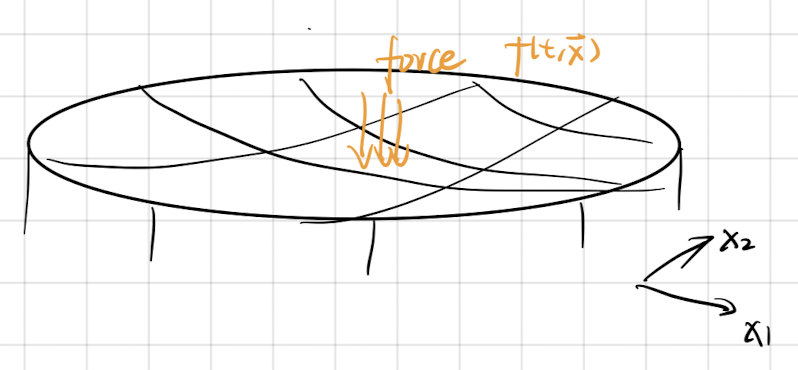
\includegraphics[width=0.5\textwidth]{membrane.png}
\caption{Diagram of the two-dimensional wave equation on a membrane.}
\end{figure}

\end{document}


\maketitle